\chapter{Evaluation}
\label{ch:eval}
In questo capitolo verranno riportati e valutati i risultati ottenuti dall’intero processo KDD.

\section{Valutazione dei risultati}

Il processo KDD terminerà con successo se si riuscirà a costruire un modello che soddisfi il task.
\subsection{KnowledgeFlow}

\begin{figure}[hbtp!]
	\centering
	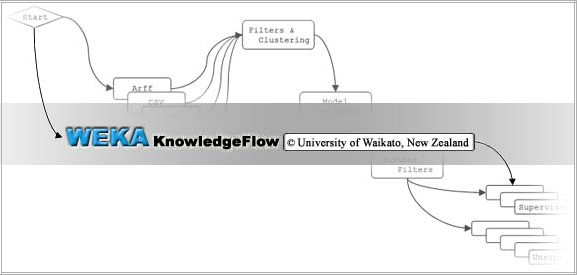
\includegraphics[width=0.6\textwidth]{./images/kf}
  	\caption{Logo di Weka KnowledgeFlow}  
\end{figure}

Per velocizzare le operazioni di confronto tra diverse tecniche di modeling si è scelto di usare lo strumento \textbf{KnowledgeFlow}, fornito sempre da Weka.

In KnowledgeFlow, l'utente può selezionare le componenti di Weka dalla barra degli strumenti, trascinarle su un canvas e collegarle l'una all'altra per formare un flusso per elaborare ed analizzare dati. Sono disponibili molti filtri, classificatori ed altri algoritmi già disponibili nell'Explorer di Weka, insieme ad altri strumenti, tipo la possibilità di salvare i risultati dell'elaborazione su un file, vedere grafici ecc.

Caratteristiche di KnowledgeFlow:
\begin{itemize}
	\item Layout intuitivo per rappresentare il flusso dei dati.
	\item Elaborazione dei dati in modalità batch o incrementale
    \item Elaborazione di più batch o stream in parallelo (ogni flusso ha il suo thread dedicato).
    \item Concatenazione di filtri.
    \item Visualizzazione delle performance dei classificatori al termine dell'elaborazione.
\end{itemize}

\subsection{Configurazioni}
Le configurazioni per la valutazione hanno visto l'utilizzo di due algoritmi, Ripper e C4.5 (rispettivamente JRip e J48 in Weka) al variare di alcuni parametri.

\begin{figure}[!htbp]
	\hspace*{-1.1in}
	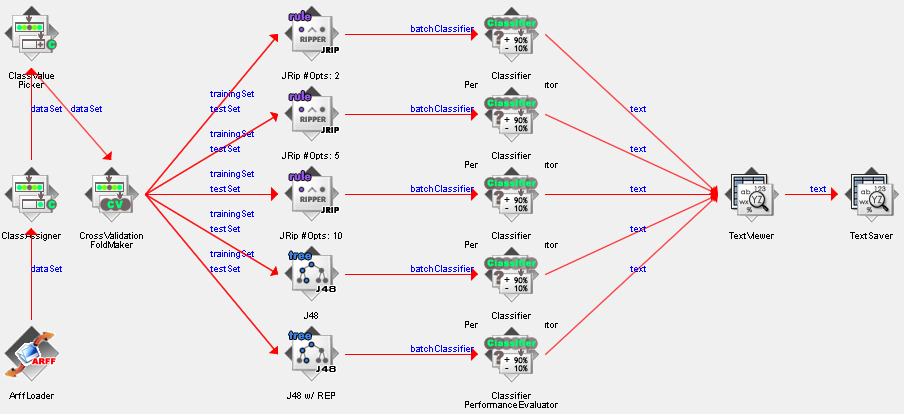
\includegraphics[width=1.4\textwidth]{./images/flow3}
\end{figure}

Nella fattispecie, le configurazioni sono:
\begin{itemize}
	\item JRip con 2 passate successive di ottimizzazione (default).
	\item JRip con 5 passate successive di ottimizzazione.
	\item JRip con 10 passate successive di ottimizzazione.
	\item J48 con pruning di default (\textit{Error-Based Pruning})\cite{Quinlan:1993:CPM:152181}.
	\item J48 con pruning effettuato da REP.
\end{itemize}
%Le varie configurazioni hanno previsto l'utilizzo di 3 tecniche di modeling, \textbf{IB1}, \textbf{Naive Bayes} e \textbf{C4.5} (quest'ultima implementata con l'algortimo J48). Ognuna ha lavorato sul dataset completo con tutti gli attributi iniziali e sulla sua versione ridotta ottenuta dalla feature selection. Inoltre per IB1 sono stati considerati diversi livelli di \emph{neighbours}, ovvero 1, 3 e 5.
%
%Questo è lo schema del workflow senza feature selection:
%
%\begin{figure}[hbtp!]
%	\hspace*{-1.1in}
%	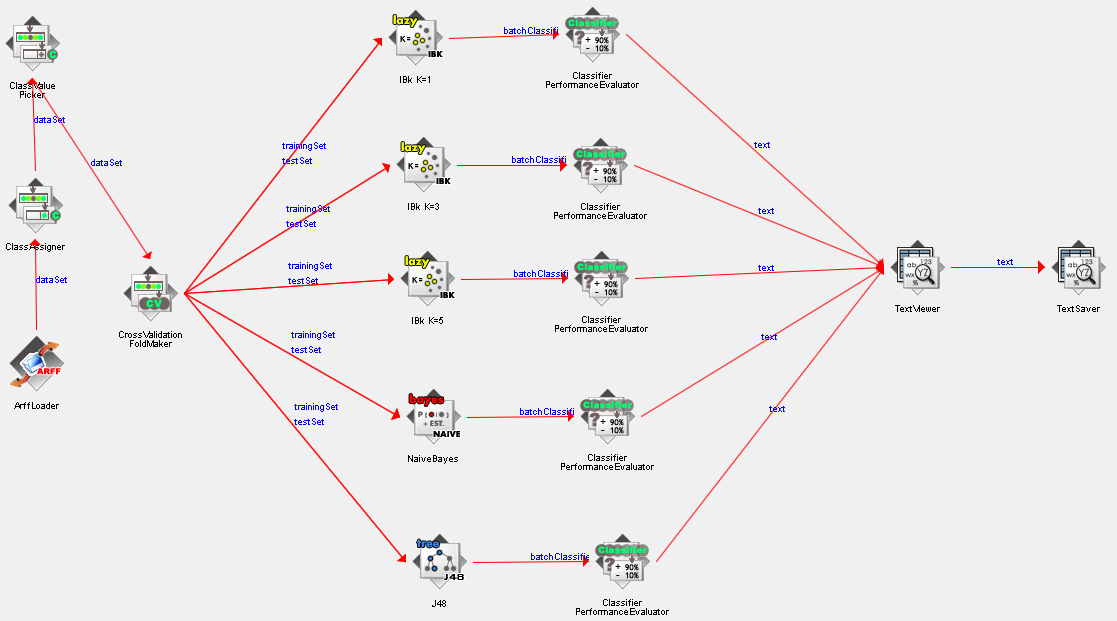
\includegraphics[width=1.4\textwidth]{./images/flow_no_featsel}
%\end{figure}
%
%Questo invece è lo schema con feature selection; l'unica differenza è la presenza della componente di filtraggio "AttributeSelection":
%
%\begin{figure}[hbtp!]
%	\hspace*{-1.1in}
%	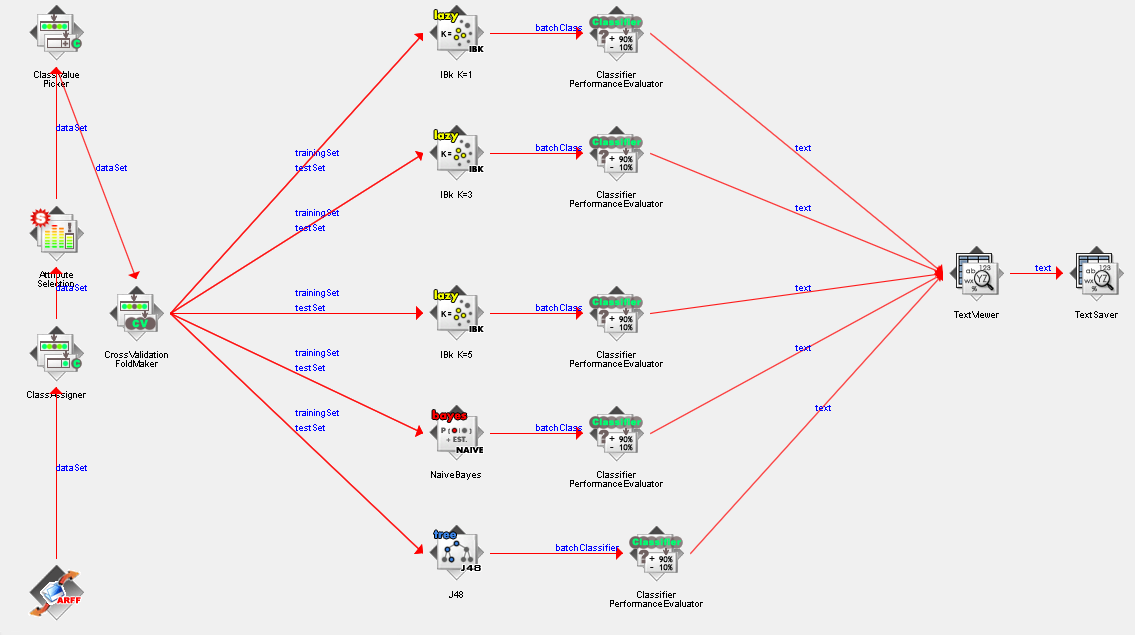
\includegraphics[width=1.4\textwidth]{./images/flow_featsel}
%\end{figure}

% \begin{sidewaysfigure}
% 	\centering
% 	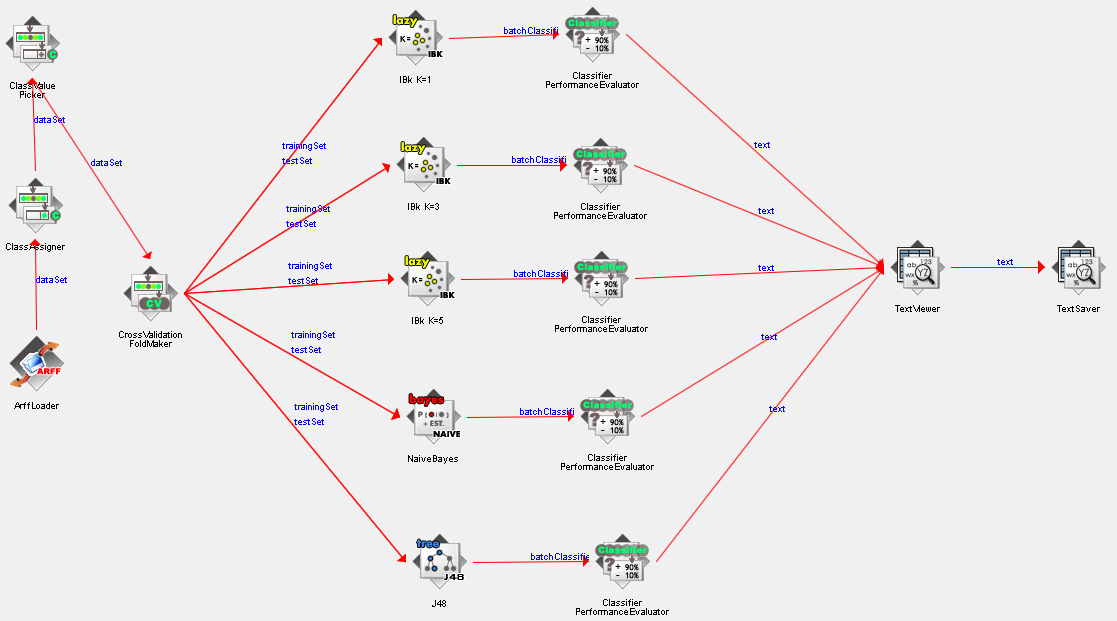
\includegraphics[width=1\textwidth]{./images/flow_no_featsel}
% \end{sidewaysfigure}

% Questo invece è lo schema con feature selection; l'unica differenza è la presenza della componente di filtraggio "AttributeSelection":

% \begin{sidewaysfigure}
% 	\centering
% 	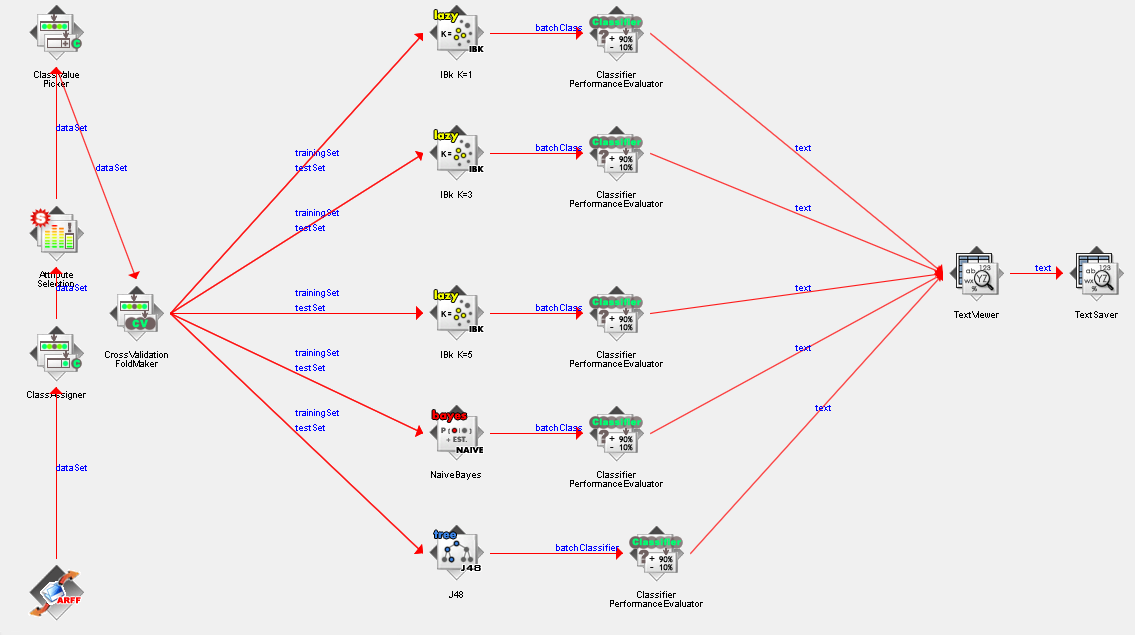
\includegraphics[width=1\textwidth]{./images/flow_featsel}
% \end{sidewaysfigure}

\subsection{Risultati delle configurazioni}
In questa sezione verranno elencati i risultati dell'esecuzione di KnowledgeFlow in base alle diverse configurazioni. \newline

%\textbf{JRip con 2 passate successive di ottimizzazione}
\vspace{0.3cm}
\begin{mdframed}[frametitle=JRip con 2 passate successive di ottimizzazione]
\begin{verbatim}
=== Evaluation result ===

Scheme: JRip #Opts: 2 : JRip
Options: -F 3 -N 2.0 -O 2 -S 1
Relation: cup98LRN


Correctly Classified Instances       16340               76.6812 %
Incorrectly Classified Instances      4969               23.3188 %
Kappa statistic                          0.5092
Mean absolute error                      0.3265
Root mean squared error                  0.4052
Relative absolute error                 65.8419 %
Root relative squared error             81.3854 %
Coverage of cases (0.95 level)          99.8123 %
Mean rel. region size (0.95 level)      88.8216 %
Total Number of Instances            21309     

=== Detailed Accuracy By Class ===

           TP Rate  FP Rate  Precision  Recall   F-Measure  ROC Area  Class
           0,492    0,004    0,990      0,492    0,657      0,746     1
           0,996    0,508    0,702      0,996    0,823      0,746     0
W. Avg.    0,767    0,279    0,833      0,767    0,748      0,746          

=== Confusion Matrix ===

a     b   <-- classified as
4766  4920 |     a = 1
49   11574 |     b = 0
\end{verbatim}
\end{mdframed}

%\textbf{JRip con 5 passate successive di ottimizzazione}

\vspace{0.5cm}
\begin{mdframed}[frametitle=JRip con 5 passate successive di ottimizzazione]
\begin{verbatim}
=== Evaluation result ===

Scheme: JRip #Opts: 5 : JRip
Options: -F 3 -N 2.0 -O 5 -S 1
Relation: cup98LRN


Correctly Classified Instances       16359               76.7704 %
Incorrectly Classified Instances      4950               23.2296 %
Kappa statistic                          0.5111
Mean absolute error                      0.3258
Root mean squared error                  0.4046
Relative absolute error                 65.7058 %
Root relative squared error             81.25   %
Coverage of cases (0.95 level)          99.8311 %
Mean rel. region size (0.95 level)      88.8193 %
Total Number of Instances            21309     

=== Detailed Accuracy By Class ===

           TP Rate  FP Rate  Precision  Recall   F-Measure  ROC Area  Class
           0,493    0,004    0,991      0,493    0,659      0,746     1
           0,996    0,507    0,702      0,996    0,824      0,746     0
W. Avg.    0,768    0,278    0,834      0,768    0,749      0,746          

=== Confusion Matrix ===

a     b   <-- classified as
4779  4907 |     a = 1
43   11580 |     b = 0
\end{verbatim}
\end{mdframed}

%\textbf{JRip con 10 passate successive di ottimizzazione}
\vspace{0.1cm}
\begin{mdframed}[frametitle=JRip con 10 passate successive di ottimizzazione]
\begin{verbatim}
=== Evaluation result ===

Scheme: JRip #Opts: 10 : JRip
Options: -F 3 -N 2.0 -O 10 -S 1
Relation: cup98LRN


Correctly Classified Instances       16374               76.8408 %
Incorrectly Classified Instances      4935               23.1592 %
Kappa statistic                          0.5126
Mean absolute error                      0.325 
Root mean squared error                  0.4042
Relative absolute error                 65.5513 %
Root relative squared error             81.1661 %
Coverage of cases (0.95 level)          99.8358 %
Mean rel. region size (0.95 level)      88.8709 %
Total Number of Instances            21309     

=== Detailed Accuracy By Class ===

           TP Rate  FP Rate  Precision  Recall   F-Measure  ROC Area  Class
           0,495    0,004    0,991      0,495    0,660      0,748     1
           0,996    0,505    0,703      0,996    0,824      0,748     0
W. Avg.    0,768    0,277    0,834      0,768    0,750      0,748          

=== Confusion Matrix ===

a     b   <-- classified as
4794  4892 |     a = 1
43   11580 |     b = 0
\end{verbatim}
\end{mdframed}

%\textbf{J48}
\vspace{0.7cm}
\begin{mdframed}[frametitle=J48 con pruning di default (EBP)]
\begin{verbatim}
=== Evaluation result ===

Scheme: J48
Options: -C 0.25 -M 2
Relation: cup98LRN


Correctly Classified Instances       14842               69.6513 %
Incorrectly Classified Instances      6467               30.3487 %
Kappa statistic                          0.3872
Mean absolute error                      0.3129
Root mean squared error                  0.524 
Relative absolute error                 63.1094 %
Root relative squared error            105.2435 %
Coverage of cases (0.95 level)          81.4398 %
Mean rel. region size (0.95 level)      65.944  %
Total Number of Instances            21309     

=== Detailed Accuracy By Class ===

           TP Rate  FP Rate  Precision  Recall   F-Measure  ROC Area  Class
           0,658    0,272    0,669      0,658    0,664      0,684     1
           0,728    0,342    0,719      0,728    0,724      0,684     0
W. Avg.    0,697    0,310    0,696      0,697    0,696      0,684          

=== Confusion Matrix ===

a    b   <-- classified as
6376 3310 |    a = 1
3157 8466 |    b = 0
\end{verbatim}
\end{mdframed}

%\textbf{J48 con pruning effettuato da REP}
\vspace{0.11cm}
\begin{mdframed}[frametitle=J48 con pruning effettuato da REP]
\begin{verbatim}
=== Evaluation result ===

Scheme: J48 w/ REP : J48
Options: -R -N 3 -Q 1 -M 2
Relation: cup98LRN


Correctly Classified Instances       16106               75.5831 %
Incorrectly Classified Instances      5203               24.4169 %
Kappa statistic                          0.4933
Mean absolute error                      0.3152
Root mean squared error                  0.4298
Relative absolute error                 63.5577 %
Root relative squared error             86.3194 %
Coverage of cases (0.95 level)          96.2457 %
Mean rel. region size (0.95 level)      84.1429 %
Total Number of Instances            21309     

=== Detailed Accuracy By Class ===

           TP Rate  FP Rate  Precision  Recall   F-Measure  ROC Area  Class
           0,562    0,083    0,850      0,562    0,677      0,762     1
           0,917    0,438    0,715      0,917    0,804      0,762     0
W. Avg.    0,756    0,276    0,776      0,756    0,746      0,762          

=== Confusion Matrix ===

a     b   <-- classified as
5448  4238 |     a = 1
965  10658 |     b = 0
\end{verbatim}
\end{mdframed}

\section{Analisi dei risultati}
Di seguito una tabella che mostra i risultati significativi delle configurazioni:

\begin{center}
\begin{tabular}{|l|c|}
	\hline
	\textbf{Configurazioni} & \textbf{Risultati} \\ \hline
	JRip con 2 passate successive di ottimizzazione (default) & 76.6812\% \\ \hline
	JRip con 5 passate successive di ottimizzazione & 76.7704\% \\ \hline
	JRip con 10 passate successive di ottimizzazione & \textbf{76.8408\%} \\ \hline
	J48 con pruning di default (EBP) & 69.6513\% \\ \hline
	J48 con pruning effettuato da REP & 75.5831\% \\ \hline
\end{tabular}
\end{center}

Come si può notare, la configurazione migliore è quella che ha previsto l'uso di JRip con 10 ottimizzazioni del ruleset con il 76.8408\% di classificazioni corrette, rispetto al 76.6812\% con solo 2 ottimizzazioni. In generale si può vedere che, ottimizzando più volte, la classificazione migliora leggermente.
Un altro aspetto interessante è dato dai risultati di J48, dove grazie al cambio del metodo di pruning, da quello di default a REP, c'è un miglioramento dal 69.6513\% al 75.5831\%, quindi un divario di quasi il 6\%, che portano la seconda configurazione di J48 ad essere competitivo con JRip.